\item The marks obtained by 30 students of Class X of a certain school in a Mathematics paper consisting of 100 marks are presented in Table \ref{table:2.1.1}
below. Find the mean of the marks obtained by the students.\\
\begin{table}[!ht]
\centering
	\input{./solutions/1-10/table/statexm/statexm1.tex}
\caption{}
\label{table:2.1.1}
\end{table}
\solution
\renewcommand{\theequation}{\theenumi}
\begin{enumerate}[label=\arabic*.,ref=\thesubsubsection.\theenumi]
\numberwithin{equation}{enumi}
\item In the given question,
\\
The sample size = Total number of possibilities(S)=6
\begin{align}
\myvec{1&2&3&4&5&6}
\end{align}
Event size= Odd number =3
\begin{align}
\myvec{1&3&5}
\end{align}
Probability for this event is = $\frac{1}{2}$
\\
The python code for the distribution of data,
\begin{lstlisting}
prob/codes/prob6_b.py
\end{lstlisting}
This shows the diagrametic representation of dice with the live update of probability with the role of dice.
\end{enumerate}

\item Table \ref{table:2.1.2}
 below gives the percentage distribution of female teachers in the primary schools of rural areas of various states and union territories (U.T.) of India. Find the mean percentage of female teachers by all the three methods discussed
in this section.\\
\begin{table}[!ht]
\centering
	\input{./solutions/1-10/table/statexm/statexm2.tex}
%\resizebox{\columnwidth}{!}{
%\begin{tabular}{|c|c|c|c|c|c|c|c|}
%\hline
%Percentage of female teachers $(x_i)$&15-25&25-35&35-45&45-55&55-65&65-75&75-85\\
%\hline
%Number of states/U.T.$(f_i)$&6&11&7&4&4&2&1\\
%\hline
%\end{tabular}
%}
\caption{}
Source : Seventh All India School Education Survey conducted by NCERT
\label{table:2.1.2}
\end{table}
\solution
From the given information, the desired equation is
\begin{align}
\norm{\vec{x}-\myvec{-3\\2}}^2 = 4^2
\\
\implies \vec{x}^T\vec{x}+\myvec{6&-4}\vec{x} -3 &=0
\end{align}
The python code for Fig. \ref{fig:4.1.1_circle} is
\begin{lstlisting}
solutions/1/codes/circle/circle1.py
\end{lstlisting}
\begin{figure}[!ht]
\centering
\includegraphics[width=\columnwidth]{./solutions/1/figs/circle/circle1.eps}
\caption{Circle using python}
\label{fig:4.1.1_circle}
\end{figure}


\item The distribution below in Table \ref{table:2.1.3}
 shows the number of wickets taken by bowlers in one-day cricket matches. Find the mean number of wickets by choosing a suitable
method. What does the mean signify?
\begin{table}[!ht]
\centering
	\input{./solutions/1-10/table/statexm/statexm3.tex}
%\resizebox{\columnwidth}{!}{
%\begin{tabular}{|c|c|c|c|c|c|c|c|c|}
%\hline
%Number of wickets &20-60&60-100&100-150&150-250&250-350&250-450\\
%\hline
%Number of bowlers &7&5&6&12&2&3\\
%\hline
%\end{tabular}
%}
\caption{}
\label{table:2.1.3}
\end{table}
\\
\solution
Let $X \in \cbrak{i}_{i=1}^{6}$ and $f_i$ be the correspnding frequency.  Then, 
\begin{align}
\pr{X=i} &= \frac{f_i}{1000}
\end{align}
The following code computes the probabilities
\begin{lstlisting}
solutions/1-10/codes/probexm/probexm3.py
\end{lstlisting}
%\begin{figure}[!ht]
%	\centering
%	\includegraphics[width=\columnwidth]{./figures/probexm/probexm3.eps}
%	\caption{probability of outcome of biased dice }
%	\label{fig:bts3}
%	\begin{lstlisting}
%	figs/probexm/probexm3.eps
%	\end{lstlisting}
%\end{figure}

\item The wickets taken by a bowler in 10 cricket matches are as follows:\\
2 6 4 5 0 2 1 3 2 3\\
Find the mode of the data.
\\
\solution
Let $X \in \cbrak{i}_{i=1}^{6}$ and $f_i$ be the correspnding frequency.  Then, 
\begin{align}
\pr{X=i} &= \frac{f_i}{1000}
\end{align}
and
\begin{align} 
\pr{X=6} &= \frac{14}{200}
\\
&= 0.07
\end{align}
The related code is available in 
\begin{lstlisting}
solutions/1-10/codes/probexm/probexm4.py
\end{lstlisting}
%\begin{figure}[!ht]
%	\centering
%	\includegraphics[width=\columnwidth]{./figures/probexm/probexm4.eps}
%	\caption{bernoulli distribution of no to be 6}
%	\label{fig:bt2}
%	\begin{lstlisting}
%	figs/probexm/probexm4.eps
%	\end{lstlisting}
%\end{figure}

\item A survey conducted on 20 households in a locality by a group of students
resulted in the following frequency table for the number of family members in a
household:
\begin{table}[!ht]
\centering
\resizebox{\columnwidth}{!}{
\begin{tabular}{|c|c|c|c|c|c|}
\hline
Family size &1-3&3-5&5-7&7-9&9-11\\
\hline
Number of families &7&8&2&2&1\\
\hline
\end{tabular}
}
\caption{}
\label{table:2.1.5}
\end{table}
Find the mode of this data
\\
\solution
In this table max frequency is 8 and modal class related to it is 3-5.
\\
\begin{align}
l &= 3
\\
h = 2
\\
f_1 &= 8
\\
f_0 &= 7
\\
f_2 &= 2
\\
Mode &= l+\frac{f_1 - f_o}{2f_1 - f_o - f_2}\times h
\\
&= 3+\frac{8 - 7}{2\times 8 - 7- 2}\times 2
\\
&=3.28
\end{align}
Related code is available in 
\begin{lstlisting}
codes/static5.py
\end{lstlisting}

\item The marks distribution of 30 students in a mathematics examination are
given in Table \ref{table:2.1.6}
Find the mode of this data. Also compare and
interpret the mode and the mean.
\begin{table}[!ht]
	\centering
	\input{./solutions/1-10/table/statexm/statexn6.tex}
\caption{}
\label{table:2.1.6}
\end{table}
\\
\solution
From the given information,
\begin{enumerate}
\item 
\begin{align}
\pr{X>9000} &= \frac{325 +445}{1000}
\\
&=0.77
\end{align}
\item 
\begin{align}
\pr{4000<X<14000} &= \frac{20+210+325}{1000}
\\
&=0.0.555
\end{align}
\item 
\begin{align}
\pr{X<4000} &= \frac{20}{1000}
\\
&=0.02
\end{align}
Related codes are available in 
\begin{lstlisting}
solutions/1-10/codes/probexm/probexm6.py
\end{lstlisting}
%\begin{figure}[!ht]
%	\centering
%	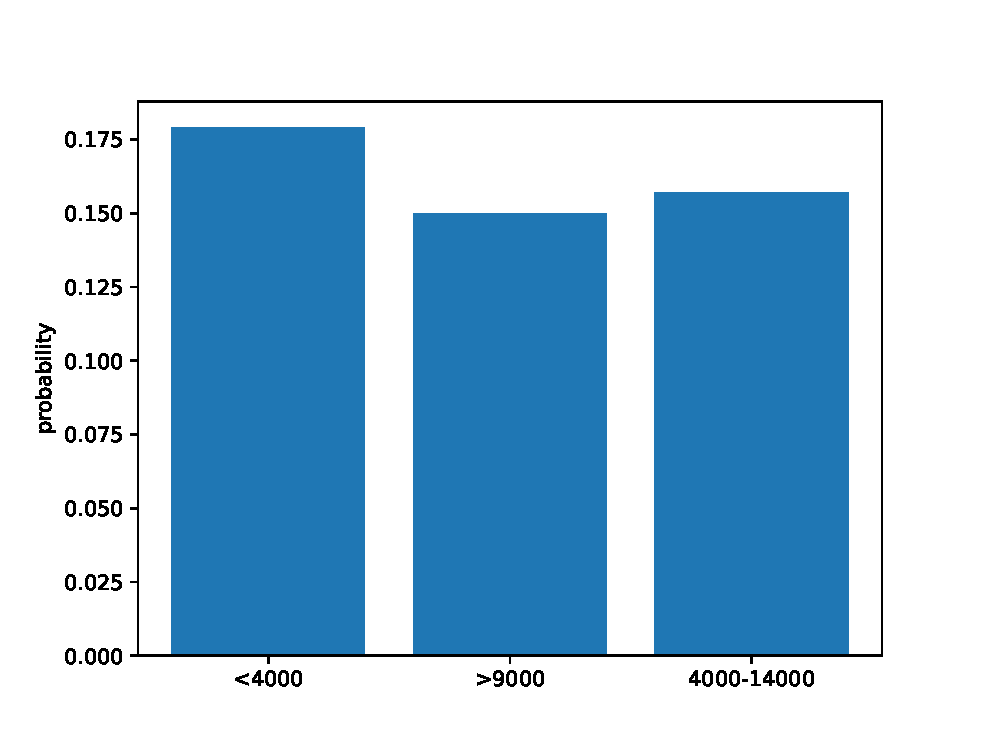
\includegraphics[width=\columnwidth]{./figures/probexm/probexm6.eps}
%	\caption{probability of distance covered by tyre }
%	\label{fig:bt6}
%	\begin{lstlisting}
%	figs/probexm/probexm6.eps
%	\end{lstlisting}
%\end{figure}
\end{enumerate}


\item A survey regarding the heights (in cm) of 51 girls of Class X of a school
was conducted and the  data in Table \ref{table:2.1.7}
was obtained.  Find the median height.

\begin{table}[!hb]
\centering
\input{./stats/tables/2.1.7.tex}
%\resizebox{\columnwidth}{!}{
%\begin{tabular}{|c|c|c|c|c|c|c|c|c|}
%\hline
%Height (in cm) &lessthan 140&lessthan 145&lessthan 150&lessthan 155&lessthan160&lessthan 165\\
%\hline
%Number of girls &41&29&40&46&51\\
%\hline
%\end{tabular}
%}
\caption{}
\label{table:2.1.7}
\end{table}
\solution
From the given information,
\begin{align}
\pr{X>70} &= \frac{3}{5}
\\
&= 0.6
\end{align}

\item The median of the  data in Table \ref{table:2.1.8}
is 525. Find the values of x and y, if the
total frequency is 100.
\begin{table}[!ht]
\centering
	\input{./solutions/1-10/table/statexm/statexn8.tex}
%\resizebox{\columnwidth}{!}{
%\begin{tabular}{|c|c|c|c|c|c|c|c|c|c|c|}
%\hline
%Class interval &0-100&100-200&200-300&300-400&400-500&500-600&600-700&700-800&800-900&900-1000\\
%\hline
%Frequency &2&5&x&12&517&20&y&9&7&4\\
%\hline
%\end{tabular}
%}
\caption{}
\label{table:2.1.8}
\end{table}
\\
\solution
Let $X \in {1,2,3}$ represent the random variable representing the age groups of the drivers. Let $Y$ represent the accidents
\begin{enumerate}
\item Then,
\begin{align}
\pr{X=1, Y = 3} &= \frac{61}{2000}
\\
&= 0.03
\end{align}
\item 
\begin{align}
\pr{X=2, Y \ge 1} &= \frac{125+60+22+18}{2000}
\end{align}
\item 
\begin{align}
\pr{Y = 0} &= \frac{440+505+360}{2000}
\\
&= 0.65
\end{align}
Related code is available in 
\begin{lstlisting}
solutions/1-10/codes/probexm/probexm8.py
\end{lstlisting}
%\begin{figure}[!ht]
%\centering
%\includegraphics[width=\columnwidth]{./figures/probexm/probexm8.eps}
%\caption{probability ofaccident in an year }
%\label{fig:bt2}
%\begin{lstlisting}
%figs/probexm/probexm8.eps
%\end{lstlisting}
%\end{figure}
\end{enumerate}

\item The annual profits earned by 30 shops of a shopping complex in a locality give rise to  the  distribution in Table \ref{table:2.1.9}.  Draw both ogives for the data and obtain the median profit.

\begin{table}[!ht]
\centering
\input{./stats/tables/2.1.9.tex}
%\resizebox{\columnwidth}{!}{
%\begin{tabular}{|c|c|c|c|c|c|c|c|}
%\hline
%Profit (Rs in lakhs) & more than or equal to 5 & morethan or equal to 10 & morethan or equal to 5&morethan orequal to 15 & morethan or equal to 20 & morethan or equal to 25 & morethan or equal to 30 & morethan or equal to 35\\
%\hline
%Number of shops (frequency)&30&28&16&14&10&7&3\\
%\hline
%\end{tabular}
%}
\caption{}
\label{table:2.1.9}
\end{table}
\solution
\begin{enumerate}
\item 
From the given information, 
\begin{align}
\pr{46<X<50} &= \frac{3}{38}
\\
&= 0.079
\end{align}

\item There is no student whose weight is less than 31 kg thus the probability of a student to have the weight less than 31 kg = 0\\

All of the student in this context  have the weight between 31-75 so we can say that the probability of the students to have the weight in the range 31-75 = 1
\end{enumerate}

        
